\documentclass[Report.tex]{subfiles}
\externaldocument[I-]{chapter_1_introduction.tex}
\externaldocument[M-]{chapter_2_method.tex}
\externaldocument[D-]{chapter_3_discardMethod.tex}
\externaldocument[C-]{chapter_5_conclusion.tex}
\externaldocument[RE-]{chapter_6_references.tex}

\begin{document}
\chapter{Result - Discussion}
\label{chap:Result - Discussion}
\section{Result: Text Segmentation}
We tried 3 Approaches, Morphological, Stroke Width Transform and OpenCv Scene text detection. We ended up with the simple solution, Morphological approach. It gives good results, but has a lot of limitations. It only works on black text with white background, images with little noise, and with text only in the image, you can see the result in figure~\ref{result:fig:Text_seg_result}. We could include a part to distinguish between text and non-text areas to improve this solution. A strategy to do that can be to compare numbers of connected components, since we know text regions have a lot of letters/components, compared to a coffee cup or a wallet.

\begin{figure}[ht]
  \centering
  \begin{subfigure}[t]{4cm}
    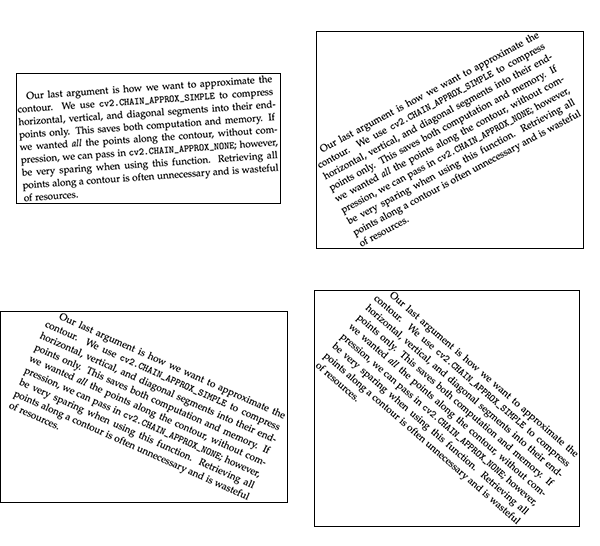
\includegraphics[width=4cm]{res/segment_text1.png}
    \caption{Good result on pure text}
  \end{subfigure}
  \hspace{7mm}%
  \begin{subfigure}[t]{4cm}
    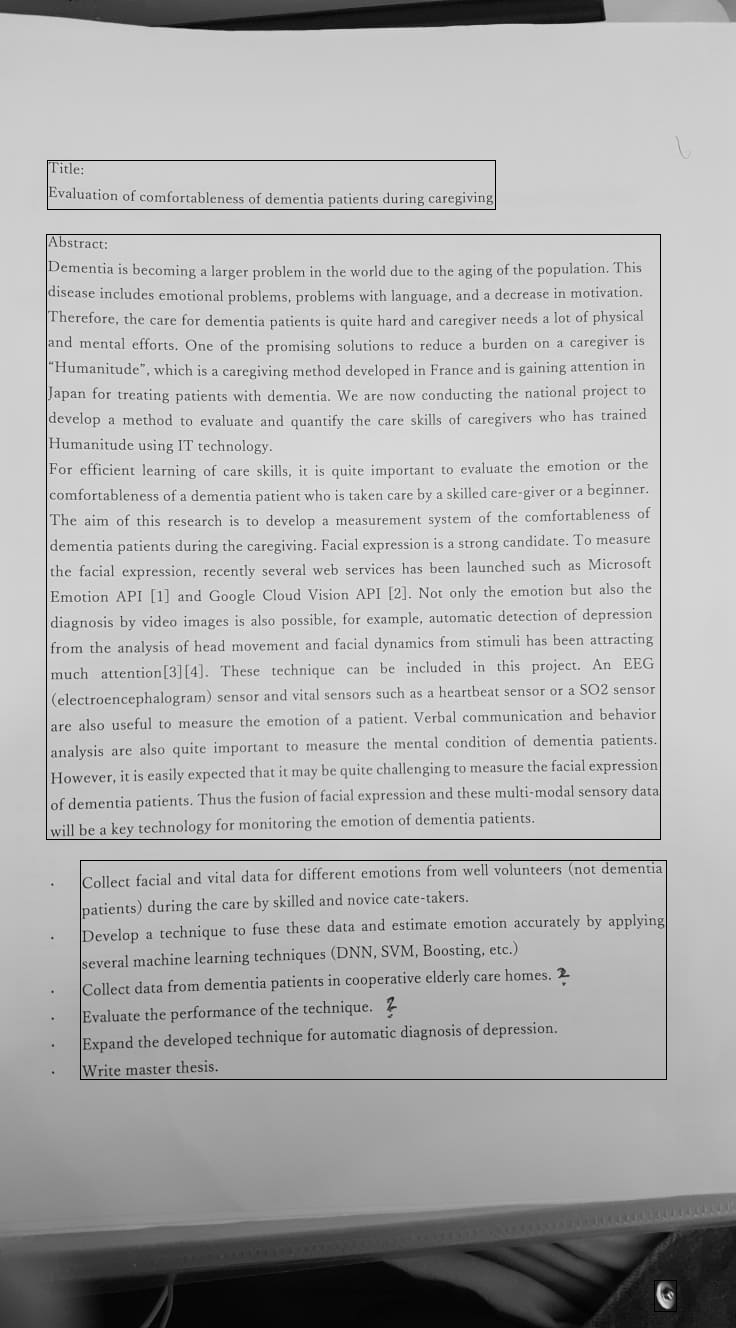
\includegraphics[width=3cm]{res/segment_text2.png}
    \caption{Good result on text on paper with little background noise}
  \end{subfigure}
  \hspace{5mm}%
  \begin{subfigure}[t]{4cm}
    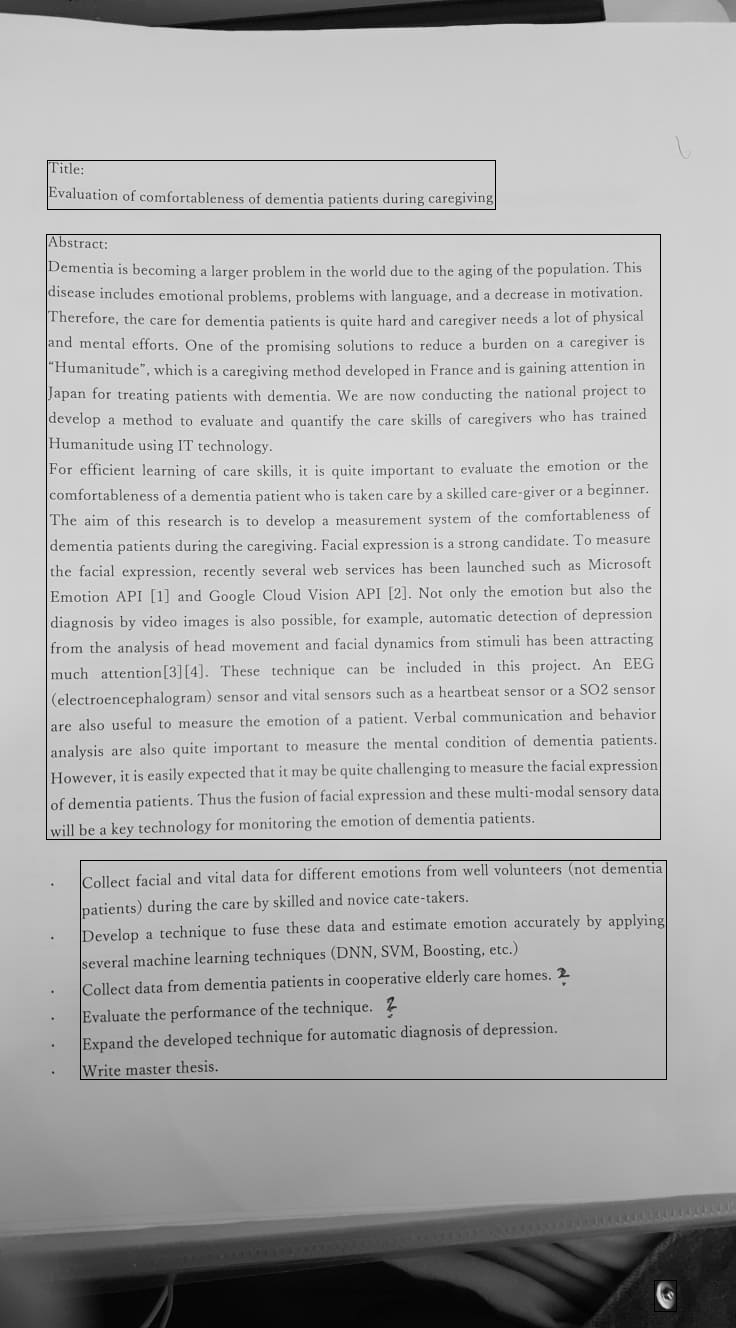
\includegraphics[width=3cm]{res/segment_text3.png}
    \caption{Bad result with many non text object segmented as text}
  \end{subfigure}
  \caption{Result of the Text Segmentation}
  \label{result:fig:Text_seg_result}
\end{figure}

\section{Result: Preprocessing}

\subsection*{Rotation}
Rotation only work if the angle of rotation is less than 45 degree. This problem is mentioned in section~\ref{Method:Preprocessing}, and an attempt to solve the problem was given in section~\ref{Discard:rotation}. Below the result of a image with rotation less than 45 degrees is showed in figure \ref{fig:result:rotation}

\begin{figure}[ht]
  \centering
  \begin{subfigure}[t]{6cm}
    \frame{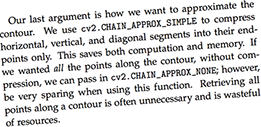
\includegraphics[width=6cm]{res/text_skew_region.png}}
    \caption{Region of skew text, after text segmentation}
  \end{subfigure}
  \hspace{2cm}%
  \begin{subfigure}[t]{6cm}
    \frame{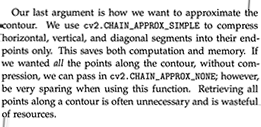
\includegraphics[width=6cm]{res/text_skew_region_rotated.png}}
    \caption{After rotation}
  \end{subfigure}

  \caption{Result of rotation}
  \label{fig:result:rotation}
\end{figure}

\subsection{Line segmentation}
If the image has no space between lines or is slightly rotated, it can cause an error, lines will not be separated. As our previous steps handles these problem our method worked quite well on our test images.
\begin{figure}[ht]
  \centering
  \begin{subfigure}[t]{6cm}
    \frame{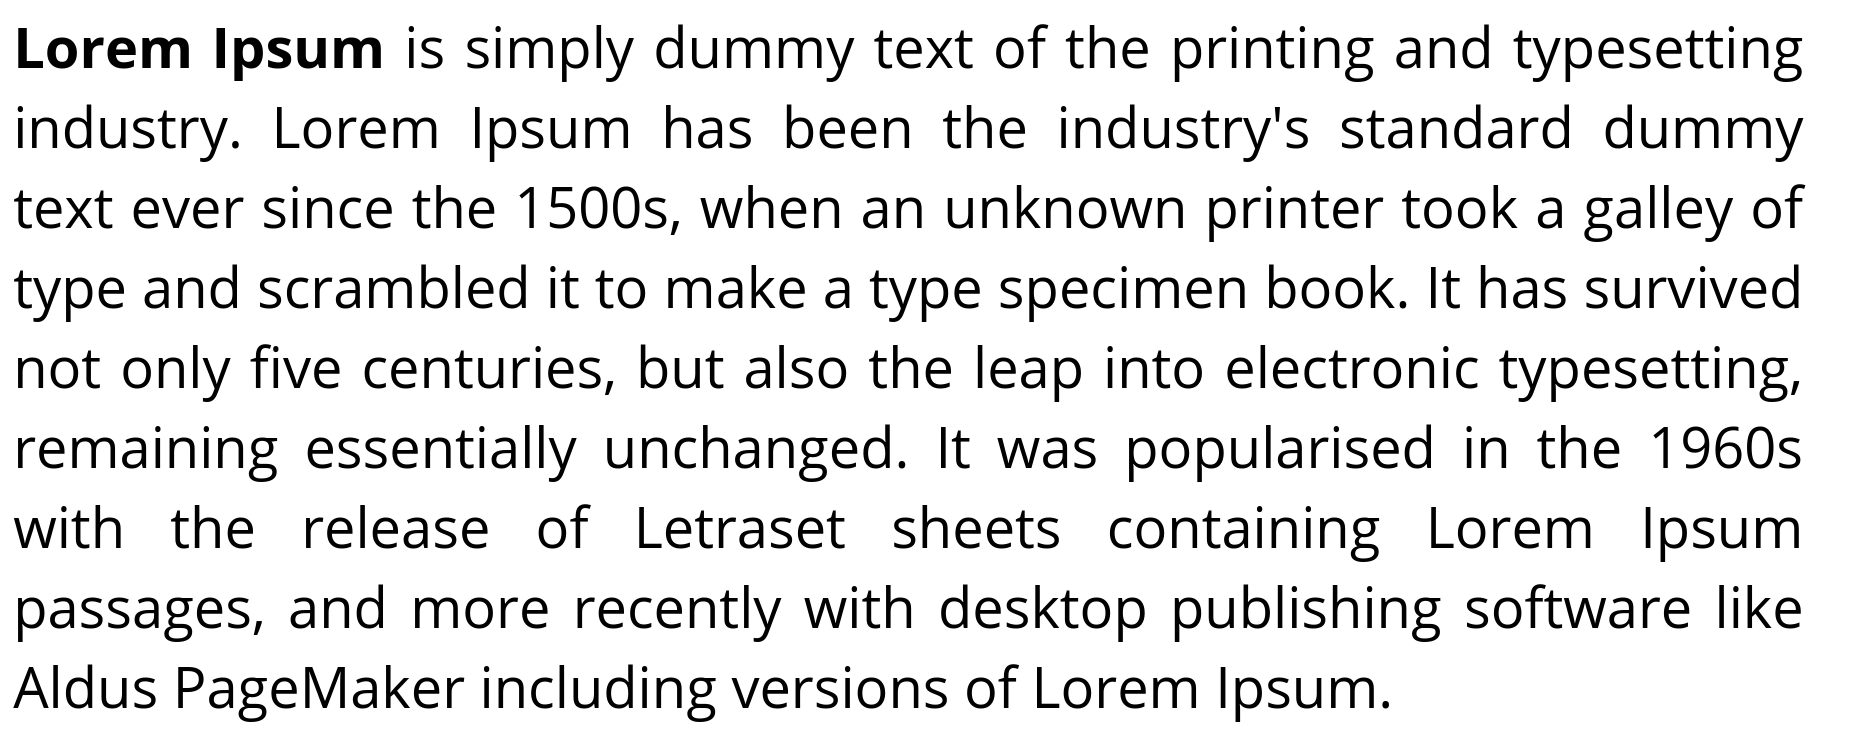
\includegraphics[width=6cm]{res/lorem_hq.png}}
    \caption{Text Region after rotation}
  \end{subfigure}
  \hspace{2cm}%
  \begin{subfigure}[t]{6cm}
    \frame{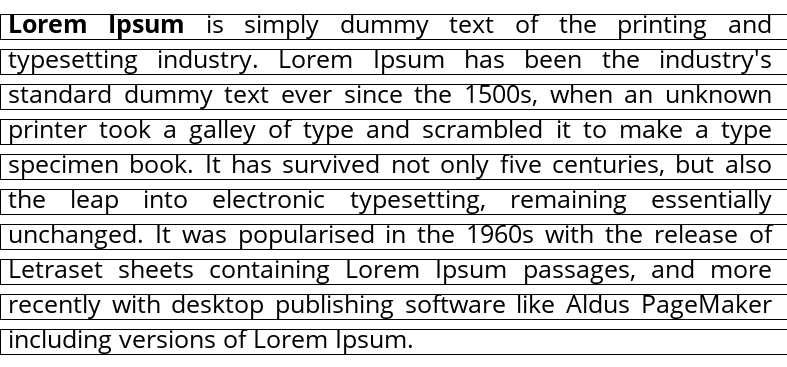
\includegraphics[width=6cm]{res/segment_line.png}}
    \caption{Boundary box of line region}
  \end{subfigure}

  \caption{Result of line segmentation}
  \label{fig:result:rotation}
\end{figure}

\subsection{Character segmentation}
\begin{flushleft}
This part worked quiet well, an alternative would be to just use OpenCv findComponent. The steps and results would not differ too much, but we could have dropped cv2.floodFills. \par
A weakness of this approach is, if multiple characters are merged with one another we would not be able to separate them. A solution for this problem can be to do a morphological opening to separate character better. Another problem we came across was we require image to be in a somewhat good quality. If image have not good enough quality it became harder to separate character from each other, as we require clear space in between them.
\end{flushleft}

\begin{figure}[H]
  \begin{subfigure}[t]{\textwidth}
    \centering
    
\includegraphics[height=0.45cm]{res/segment_letter1.png}
    \caption{Result of Character Segmentation from extracted line}
  \end{subfigure}
  \begin{subfigure}[t]{\textwidth}
    \centering
    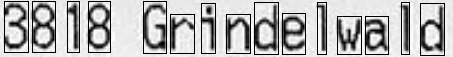
\includegraphics[width=12cm]{res/segment_letter2.png}
    \caption{Result of Character Segmentation from an example line image}
  \end{subfigure}
  \caption{Result of Character segmentation}
  \label{fig:Character_segmentation}
\end{figure}



\section{Result: Classification}
\subsection{Description}
\begin{flushleft}
  Convolutional neural networks are especially good for image
  classification, because they take local spatial connections into account when
  they classify. This way it doesn't matter where in the image our
  object/character is it will be able to recognize it, same yields for rotation,
  as the CNN classifies based on local spatial connections it doesn't matter if
  the object is slightly rotated. Hence the classification would be even more robust compared to the MLP.\par
  
  Following figures show topology and performance during training.
  Topology stays the same as described in Figure \ref{fig_topology}.
  In Figure \ref{fig_accuracy} we can observe how the accuracy changes over time.
  You can notice drastic acceleration after 2'000 steps, this is due to us changing the dataset context as we used multiple independent datasets during one training session.
  Loss graph \ref{fig_loss} swings follow expected path and resemble pretty much every loss graph for correctly setup network, be it MLP, CNN or any other.
  
  The final accuracy we were able to get is \textbf{87.76\%} and it only took us approximately 30 min of training on \textbf{nVidia GeForce 840M GPU}.
\end{flushleft}

\begin{figure}[!htb]
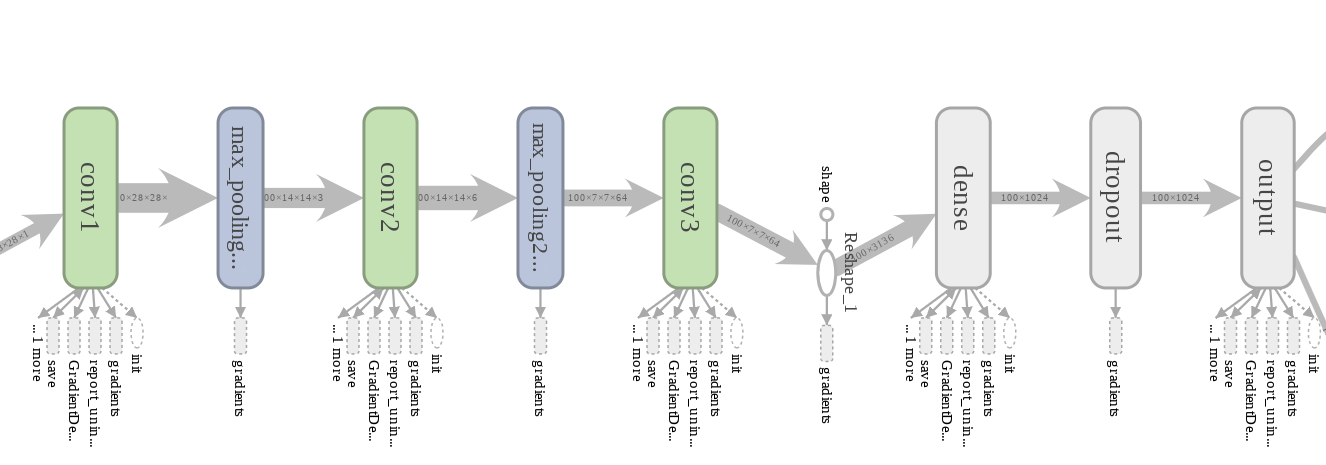
\includegraphics[width=\textwidth]{res/topology.png}
\caption{CNN topology}
\label{fig_topology}
\end{figure}

\begin{figure}[!htb]
  \begin{subfigure}[t]{\textwidth}
    \centering
    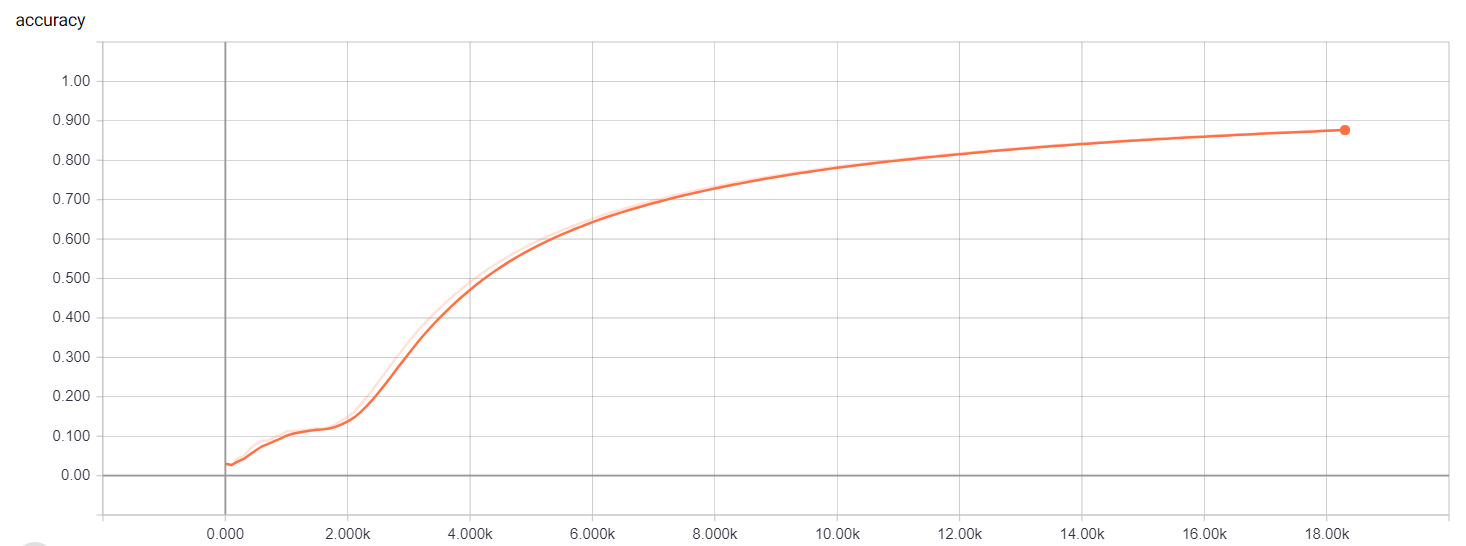
\includegraphics[width=\textwidth]{res/accuracy.png}
    \caption{Accuracy during training}
    \label{fig_accuracy}
  \end{subfigure}
  \begin{subfigure}[t]{\textwidth}
    \centering
    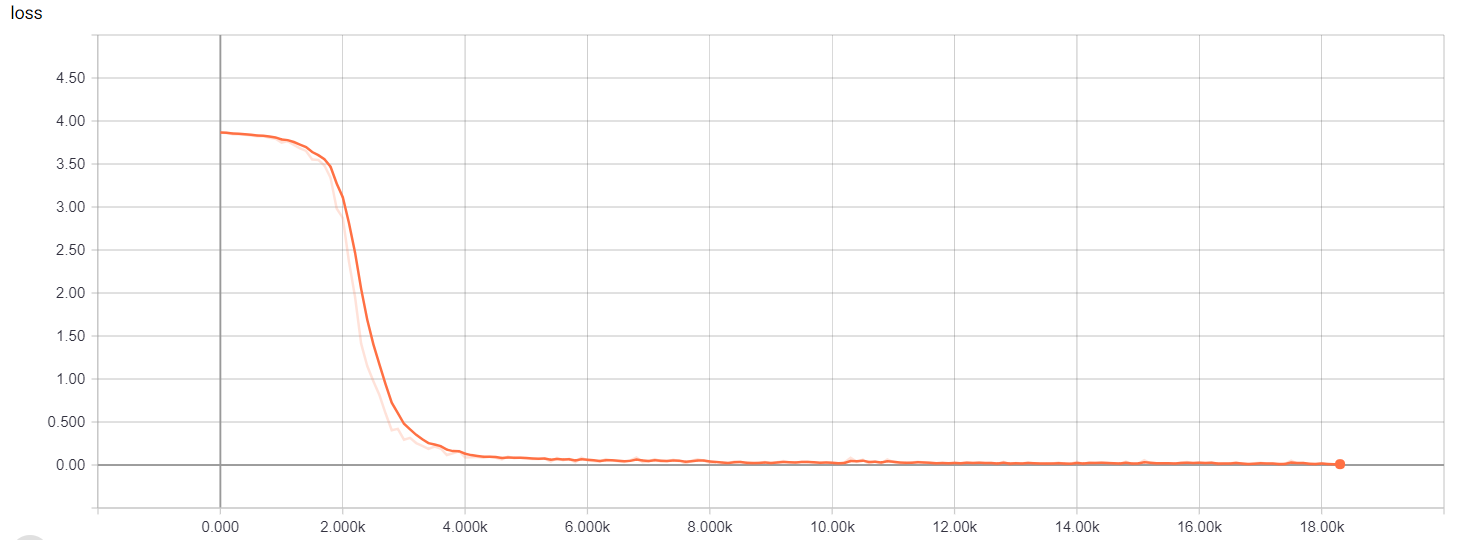
\includegraphics[width=\textwidth]{res/loss.png}
    \caption{Loss graph during training}
    \label{fig_loss}
  \end{subfigure}
  \caption{Result of Classification}
  \label{fig:Character_segmentation}
\end{figure}

On Figure \ref{fig_filter_view} we can see what some filters see on an image. Each image shows what one of filters in each convolutional layer can see. Image to the left is filter from conv1 layer, middle from conv2 layer and last one from conv3 layer.\\
For example we can observe that filter in the middle has brighter colors when is 'sees' vertical lines, while first and last filters detect left edges of the object.

\begin{figure}[!htb]
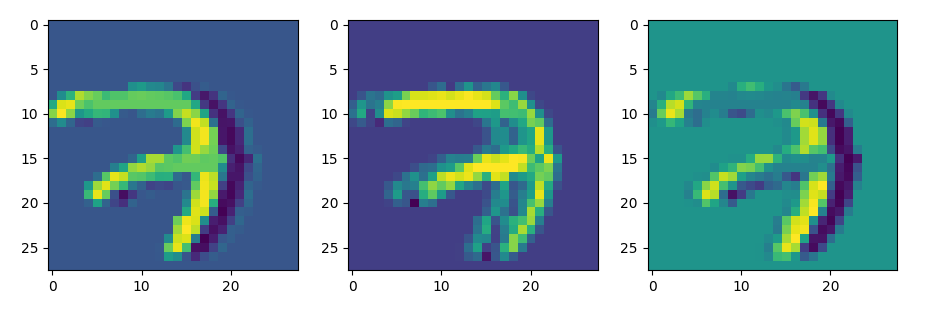
\includegraphics[width=\textwidth]{res/filter_view.png}
\caption{Filter activation}
\label{fig_filter_view}
\end{figure}

\newpage
\section{Final Result}
We saw that each component was able to its part reasonably. Each have weakness and fails, but if we are to combine them together we are able to do get a somewhat reasonable result. Figure \ref{fig:Result:Final_result} show an input image and what we got in the output. Some of the letter are not able to be classify correctly. The main error came from classification part, but we got somewhat readable result... As mention earlier we require an image with reasonably high resolution 

\begin{figure}[H]
  \begin{subfigure}[t]{\textwidth}
    \centering
    \frame{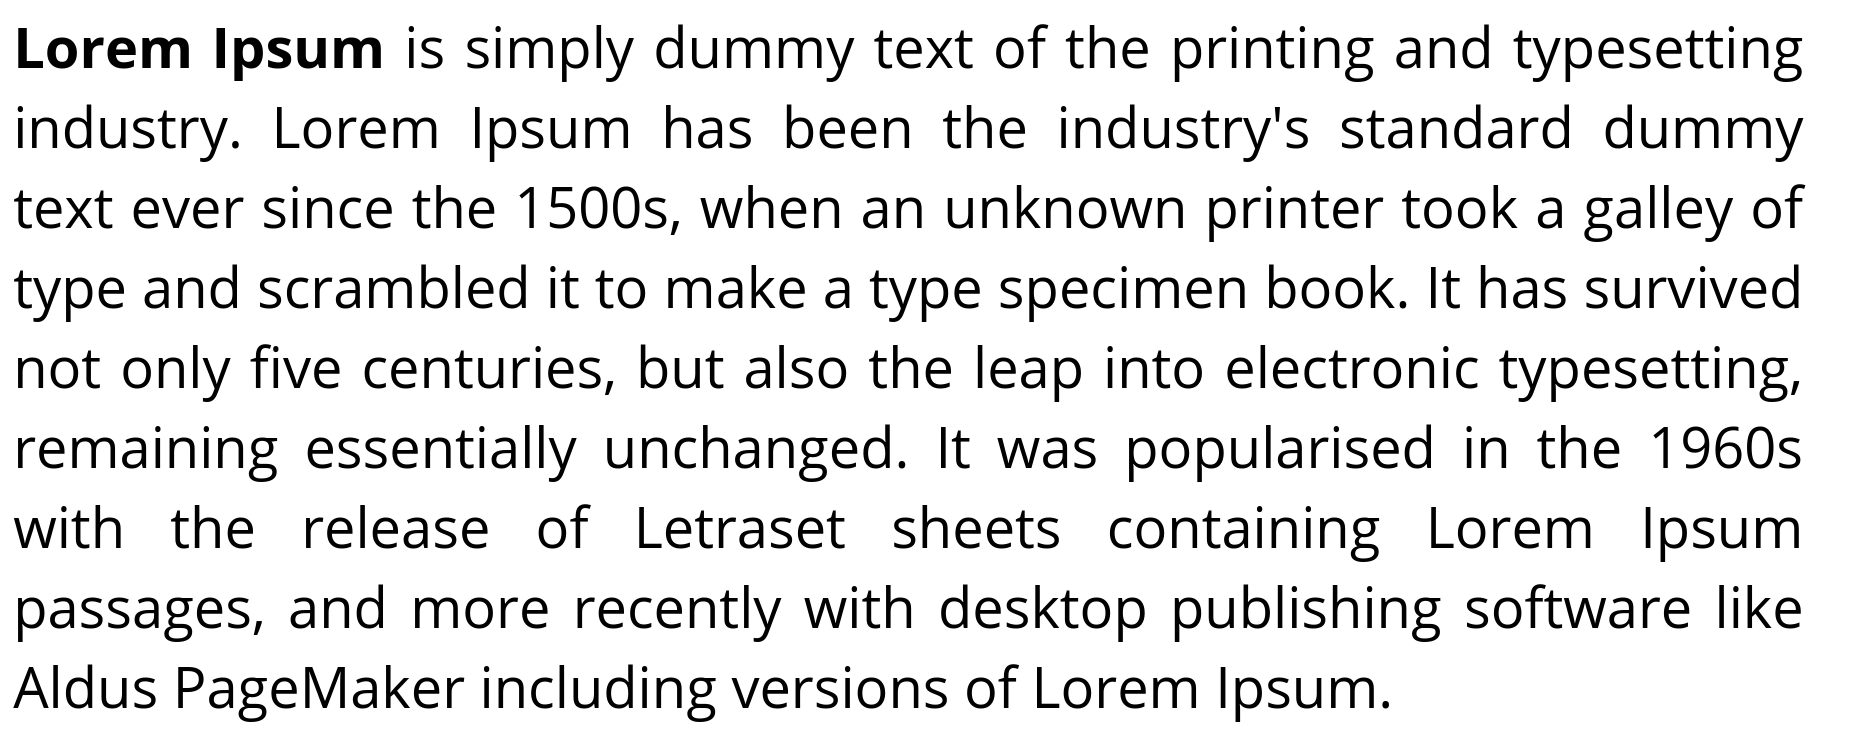
\includegraphics[width=12cm]{res/lorem_hq.png}}
    \caption{Original image 'lorem.png' as input image}
  \end{subfigure}
  \begin{subfigure}[t]{\textwidth}
    \centering
    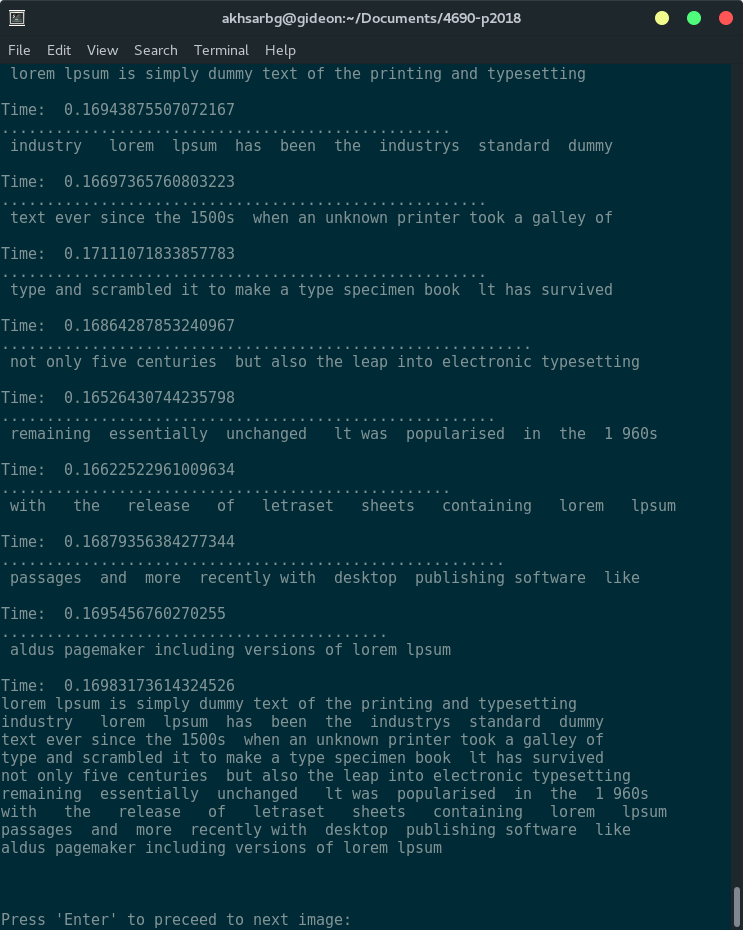
\includegraphics[width=12cm]{res/lorem_output.png}
    \caption{Terminal output of lorem.png}
  \end{subfigure}
  \caption{Final Result of lorem.png}
  \label{fig:Result:Final_result}
\end{figure}

\end{document}
